\section{Effect of noise on Equations~\eqref{2302:eq:def:gf_ode}}

\label{2302:app:noise-term}
In this appendix we present some corrective terms to Equations~\eqref{2302:eq:def:gf_ode} that allows to have better results when numerically integrating ODEs and comparing them to simulations.

In \cite{veiga2022phase} the terms proportional to $\sfrac{\lr}{\hids}$ are neglected completely when running numerical integrations. However, we noticed that a term from $\Psi^{(\mathrm{Var})}_{ij}(\Omega)$ could be kept in order to get better agreement between ODEs and simulation in presence of label noise at small but finite $\sfrac{\gamma}{p}\ll 1$.
Letting \(\mathcal{E}^*  \coloneqq \mathcal{E} - \sqrt{\noise}z\), we can decompose
\[
    \Psi^{(\mathrm{Var})}_{ij}(\Omega) = \mathbb E_{(\vec{\lambda},\vec{\lambda}^{\star})\sim\mathcal{N}(\vec{0}_{\hids+\hidt}, \Omega)} \left[\sigma'(\lambda_i)\sigma'(\lambda_j)\,{\mathcal{E}^*}^2 \right] + \mathbb E_{(\vec{\lambda},\vec{\lambda}^{\star})\sim\mathcal{N}(\vec{0}_{\hids+\hidt}, \Omega)} \left[\sigma'(\lambda_i)\sigma'(\lambda_j)\,\noise \right],
\]
allowing us to define
\begin{equation}
    \Psi^{(\mathrm{noise})}_{ij}(\Omega) \coloneqq \mathbb E_{(\vec{\lambda},\vec{\lambda}^{\star})\sim\mathcal{N}(\vec{0}_{\hids+\hidt}, \Omega)} \left[\sigma'(\lambda_i)\sigma'(\lambda_j)\,\noise \right].
\end{equation}
The asymptotic of this term at late times $t\gg 1$ was explicitly computed in \cite{biehl1995learning} and \cite{goldt2019dynamics} for different architectures, where it was found that $\Psi^{(\mathrm{noise})}_{ij} \propto \noise$. In these cases, when the dynamics approaches the point where \(\mathcal{E}^* \sim \sfrac{\lr\noise}{\hids}\), then the term $\Psi^{(\mathrm{GF})}_{ij}(\Omega)$ is of the same order of $\sfrac{\lr}{\hids}\Psi^{(\mathrm{noise})}_{ij}(\Omega)$, while the remaining part of $\Psi^{(\mathrm{Var})}_{ij}(\Omega)$ is still negligible since is scaling as \({\mathcal{E}^*}^2\). 
It follows that the first order correction in $\sfrac{\gamma}{p}$ of equations \eqref{2302:eq:def:gf_ode} is given by: 
\begin{align}
\tag{GF-ODE-NOISE}\label{2302:eq:def:ode_gf_withnoise}
\frac{\dd\mat{M}}{\dd t} = \Psi^{(\mathrm{M})}(\Omega), && \frac{\dd\mat{Q}}{\dd t} =  \Psi^{(\mathrm{GF})}(\Omega) + \frac{\lr}{\hids}\Psi^{(\mathrm{noise})}(\Omega).
\end{align}
Despite vanishing in the true $\sfrac{\gamma}{\hids}\to0^+$ limit, the new term enables ODE to catch the behaviour for large times, when simulating small but finite \(\sfrac{\gamma}{p}\). 

\begin{figure}
    \centering
    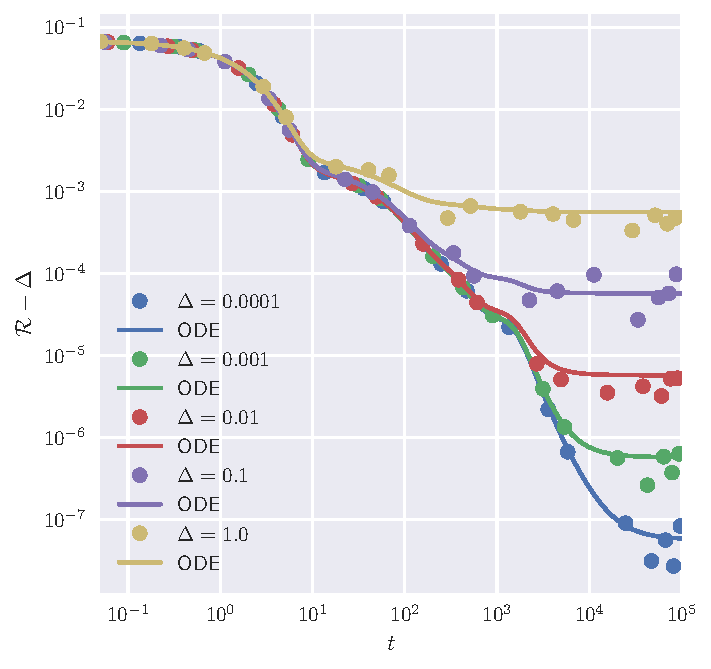
\includegraphics[width=.5\textwidth]{figs/classic/classic_limit_noises_plot_-k4_p8_d10_gamma0.0500}

    \caption{
    comparison between the  simulated learning dynamic and the one obtained by integrating the differential equations, in the \emph{classical regime}; \(\hidt=4,\hids=8,\lr=\num{5e-2},d=10, \sigma=\erf(\sfrac{\cdot}{\sqrt{2}})\). Learning the same teacher with different level of noise.
    }
    \label{2302:fig:classic-limit-noise}
\end{figure}

Figure~\ref{2302:fig:classic-limit-noise} shows a numerical experiment explicitly designed to show the effect of noise term. 
The fluctuations visible in the final plateaus result from the stochastic process in Equation~\eqref{2302:eq:def:overlap_process}: 
\(\Psi^{(\mathrm{Var})}\) and consequently \(\Psi^{(\mathrm{noise})}\) are proportional to \(\sfrac{||\vec{x}^{\i}||_{2}^{2}}{d}\). When \(d=O(1)\) then this term is not concentrating to 1 and leads to a fluctuation. 
Let us again stress the fact that this is an effect visible only when performing numerical experiments with finite GP, whereas in the true limit the fluctuations disappear and the dynamic is described by deterministic ODEs.
% %%%%%%%%%%%%%%%%%%%%%%%%%%%%%%%%%%%%%%%%%%%%%%%%%%%%%%%%%%%%%%%%%%%%%%%%%%%%%%%
